\chapter{Results and Discussion}\label{sec:results}
For every \acl{p} assay, predictions were performed by using the \ac{cp} descriptors first, then the \ac{ecfp} descriptors and eventually by using the combined feature engineered descriptors. Additionally, to validate the feature selection, another prediction run was conducted using the complete feature space, i.e. all 2048 \ac{ecfp} features and 1768 \ac{cp} features.\\
The first section compares the performance of \ac{cp} descriptors against the \acp{ecfp} among all \ac{p} assays. The second section adds the results from the modelling approach using the feature engineered data set. A comparative analysis is conducted that compares the resulting performance with those from the first and second prediction run (using \ac{cp} data or \acp{ecfp}). The fourth prediction run is then evaluated. Several metrics are compared against the feature engineered approach to validate the advantages of feature engineering.\\
An enrichment method is introduced that uses feature engineering information to connect the performance within an assay group to cellular morphology. Additionally, phenotypic keywords are manually generated to describe cellular processes concerning \ac{p} assays. The enrichment of specific keywords within assays grouped by their performance relates cellular processes to the predictive capabilities of \ac{cp} descriptors. The phenotypic keywords suffer from a limited understanding of cellular processes and can, therefore considered biased. Even though they were generated before the performance results for each assay were generated.\\
A very similar intention is pursued by the final enrichment method. Thereby, \ac{go} terms are assigned to each gene product featured in the \ac{p} assays. The \ac{go} also correspond to cellular processes and molecular functions with the difference that complete hierarchies of terms are available for a specific protein target. Enrichment of \ac{go} terms can link the predictive capabilities of \ac{cp} descriptors to cellular mechanisms similar to the phenotypic annotations but with significantly less expert bias.
\section{Comparative Analysis of ECFP and CP Predictions}\label{sec:companalyfpcp}
% intro 
The predictions were performed individually for each assay resulting in individual metrics that are compared among different descriptor sets. The first prediction run and the second prediction run are compared first. They use substantially different inputs, \ac{cp} and \ac{ecfp} descriptors, to predict the same bioassay targets. First, three performance metrics are evaluated: the \ac{auc}, \ac{ba} and \ac{mcc}. The results of both runs are presented in \fref{fig:absperffpcp}. \fref{fig:absperffpcp}a contains the \ac{auc} and b and c contain the \acl{ba} and \acl{mcc}. The results from \ac{ecfp} and \ac{cp} predictions are plotted in the same panel for the same metric. The \acl{p} assays are ordered by their \ac{auc}. Thus, assays which exert high predictive potential with \ac{cp} data are listed first. This order is kept throughout this chapter.\\
% describe a and mention most important trends of a
The \ac{cp} prediction run yielded \acp{auc} from \num{0.4} to \num{0.8} as shown in \fref{fig:absperffpcp}a. The \ac{cp} dscriptors outperform the \acp{ecfp} for 14 bioassays namely 720532, 651635, 624297, 2330, 743014, 588855, 743012, 624296, 743015, 1578, 504444, 651744, 1688 and 651610. However, 1688 and 651610 score an \ac{auc} below \num{0.7}. The remaining 12 \acl{p} assay are henceforth referred to as \acl{hpa}. All other \acl{p} assays are referred to as \acl{lpa}. In general, the \acp{ecfp} perform well with 27 \ac{auc} scoring higher than \num{0.7}.\\
% describe b mention most important trends of b
In \fref{fig:absperffpcp}b the \acl{ba} is shown for all assays. The \acl{ba} is calculated by means of the specificity and the sensitivity (see \fref{eq:balacc}). Measured by \acl{ba}, several assays perform better or worse compared to their \ac{auc}. However, the \acl{hpa} are still better scoring compared to the \acl{lpa}. The \ac{ecfp} predictions exhibit no apparent trends. However, they do not score a \acl{ba} higher than \num{0.7} which is achieved by most (83\%) of the \acl{hpa} when they are predicted using \ac{cp} data.\\
% describe c and mention most important trends of c
For the \ac{cp} predictions the \acl{mcc} is not as consistent throughout the \acl{hpa} (see \fref{fig:absperffpcp}c). The performances fluctuates from \num{0.2} to \num{0.6} depending on the assay. Five out of twelve achieve a \acl{mcc} higher than \num{0.4}. Within the \acl{lpa} the \ac{cp} predictions score very low. The trend is almost monotonously descreasing, mimicing the scoring by the \ac{auc}. A familiar trend is presented by the \acp{ecfp}. They score worse within the \acl{hpa} but better within the \acl{lpa} given a few exemptions. None of the \ac{ecfp} predictions score a \acl{mcc} higher than \num{0.4}.\\
\begin{figure}[H]
	\centering
	\includegraphics[width=\textwidth]{figures/cp_fp_comparison.pdf}
	\caption[Performance Comparison of \ac{cp} and \ac{ecfp} Predictions]{Performance comparison of \ac{cp} and \ac{ecfp} predictions. The \ac{auc}, \acf{ba} and \acf{mcc} are being compared in three bar plots. The \ac{cp} predictions are shown in purple and \ac{ecfp} in yellow with narrower bars. The \acl{p} AIDs are listed on the y-axis. Two supporting lines are drawn in each subplot. One horizontal line segregates high and \acl{lpa} and the vertical lines marks the threshold for high performance in each metric.}
	\label{fig:absperffpcp}
\end{figure}\noindent
% draw a conclusion
The first two prediction runs allowed to categorize the \acl{p} assays. A few performed consistently better via \ac{cp} descriptors, and for others, the \acp{ecfp} showed higher predictive potential. Especially for \acl{ba} and \acl{mcc}, two metrics that are more sensitive to label imbalance, the predictivity of \ac{cp} descriptors was distinguished among the \acl{hpa}. This finding can have many reasons since \ac{cp} data and \acp{ecfp} are substantially different. However, one explanation might be rooted in \ac{smote}. This oversampling strategy is reported to perform better on numerical data, as provided by \ac{cp} features. The \ac{ecfp} features, on the other hand, are boolean and therefore less suitable.\\

\section{Comparative Analysis of Modelling with Selected Features}\label{sec:companalySF}
%intro
The third prediction run was based on a mixed feature set containing \ac{cp} as well as \ac{ecfp} descriptors selected as described in \fref{sec:features}. This set of features will be referred to as \acl{sf}. When comparing the \ac{cp} and \ac{ecfp} with the \acl{sf} evaluation, the \acl{sf} are expected to overcome the shortcomings of each identifier. By closely inspecting each metric's differences and revealing unexpected trends, further information about each identifier's shortcomings and strengths can be gained.
% AUC a
The first panel in \fref{fig:diffauc} shows the assay-wise difference between the \ac{cp} and \ac{ecfp} descriptors that was shown in absolute values in \fref{fig:absperffpcp}a. Again, the \acl{hpa} are clearly distinguished by their scoring, compared to the \acl{lpa}. This figure quantifies the difference in \ac{auc} scoring between \ac{cp} and \ac{ecfp} with up to \SI{20}{\percent} greater results for AID 624297. On the other hand AID 1030 performes 30\% worse when predicted with \ac{cp}.\\
% AUC b
The comparison between \acl{sf} and \ac{ecfp} exhibits a very similar trend. The \acl{hpa} score very similar, on the other hand the \acl{lpa} score not as low. They perform up to 20\% worse, in the case of AID 1030. Also, some assays that have a negative difference in the left panel score positive, i.e. better than \acp{ecfp} when predicted with \acl{sf} (AIDs 588852, 720635 and 2156).\\
% AUC c
The range on the x-axis in \fref{fig:diffauc}c is the narrowest indicating more subtle changes when switching from \ac{cp} to \acl{sf}. The \acl{hpa} present mixed differences. Some assays are better predicted with \ac{cp} descriptors only (e.g. 651744) and others are better predicted with the \acl{sf} (e.g. 720532). For that reason, the specific effect that the combination exerts on \acl{hpa} remains inconclusive. Almost all \acl{lpa} perform better when \acl{sf} are used for modelling. The only exemption is AID 1688. The improvements within the other \acl{p} assays are as high as 20\%.\\
\vspace{-0.35cm}
\begin{figure}[H]
	\centering
	\includegraphics[width=0.9\textwidth]{figures/AUCComparison.pdf}
	\caption[Difference in AUC Between the \ac{cp}, \ac{ecfp} and \acl{sf}]{Difference in AUC between the \ac{cp}, \ac{ecfp} and \acl{sf} for all 52 \acl{p} assays. The dashed green line separates high and \acl{lpa}. The performance metrics of the right descriptor set is subtracted from the ones of the left descriptor set (as seen in the figure titles) to obtain the corresponding differences.}
	\label{fig:diffauc}
\end{figure}\noindent
% draw a conclusion
The process of features engineering fosters expectations on improvements in predictive capability and complementation of \ac{cp} and \ac{ecfp} descriptors. The process of feature engineering Inspecting the \ac{auc} comparison to \ac{cp} Improvements achieved within the \acl{lpa} of \fref{fig:diffauc}c can be attributed to the complementary information supplied by the \ac{ecfp} features from feature engineering. However, no apparent improvements can be found within the \acl{hpa} when comparing \acl{sf} to \ac{cp} as well as within the \acl{lpa} when comparing the \acl{sf} to \acp{ecfp}. This infers, that the feature selection process, might have removed descriptors that were vital for the \ac{ecfp} performance on \acl{lpa} and \ac{cp} performance on \acl{hpa}.\\
% intro
To solidify the findings drawn from \fref{fig:diffauc} further metrics are compared and analyzed. The \acl{ba} takes \ac{tnr} and \ac{tpr} into account and the descriptor comparison is shown in \fref{fig:diffbalacc}.\\
% BA a
Qualitatively the \acl{ba} between \ac{cp} and \ac{ecfp} in \fref{fig:diffbalacc} shows the same trend as seen before. The \ac{ecfp} perform slightly worse which can also be seen in \fref{fig:absperffpcp}b. The worst drop in \acl{ba} is presented by 1030 with 20\%. Furthermore, seven \acl{lpa} score higher \aclp{ba} using \ac{cp} instead of \ac{ecfp}. The difference for \acl{hpa} is almost identical to the difference in \ac{auc} concerning \ac{cp} and \ac{ecfp} comparison.\\
% BA b
The \acl{sf} compared to the \ac{ecfp} achieves consistently positive results within the \acl{hpa} and mostly negative results for the \acl{lpa}. Even though the scoring within \acl{lpa} is slightly higher compared to the \ac{auc} with eight assays that perform better using the engineered features.\\
% BA c
In \fref{fig:diffbalacc}c the difference for \acl{ba} between \ac{cp} data and \acl{sf} is shown. This panel shows the highest variation compared to the \ac{auc} scoring. The superiority of \ac{sf} within the \acl{lpa} is less definitive and the \acl{hpa} lean more towards the \ac{cp} as descriptors of choice, too. Within the \acl{lpa} there are nine assays with a lower score using \acl{sf}. Then again, AID 651744 within \acl{hpa} diminishes by 8\% after feature engineering.
\begin{figure}[H]
	\centering
	\includegraphics[width=0.9\textwidth]{figures/BalAccComparison.pdf}
	\caption[Difference in \acl{ba} Between the \ac{cp}, \ac{ecfp} and \acl{sf}]{Difference in \acl{ba} between the \ac{cp}, \ac{ecfp} and \acl{sf} for all 52 \acl{p} assays. The dashed green line separates high and \acl{lpa}. The performance metrics of the right descriptor set is subtracted from the ones of the left descriptor set (as seen in the figure titles) to obtain the corresponding differences.}
	\label{fig:diffbalacc}
\end{figure}\noindent
% draw a conclusion
Even though very similar trends can be observed for the \acl{ba} as for the \ac{auc}, the findings from the \acl{ba} incentivize a stronger objection against the \acl{sf}' capabilities since \ac{cp} data obtains better overall scores within \acl{hpa} and \acl{lpa}. Also, the margin between \acl{sf} and \ac{ecfp} for \acl{ba} is still significantly large even if it is slightly smaller compared to the \ac{auc} comparison in \fref{fig:diffauc}b.\\
% intro
The \acl{mcc} is a performance metric that is sensitive to label imbalance. This metric is consulted to confirm the findings in the \acl{ba} comparison.\\
%MCC a
The differences between the \ac{ecfp} and \ac{cp} descriptors mirror \fref{fig:diffbalacc}a. The \acl{hpa} in \fref{fig:diffmatcff}a score higher with \ac{cp} data opposed to \acl{lpa} which score generally better with \acp{ecfp}, apart from a few exemptions that are in agreement with the exemptions found for the respective \acl{ba} comparison.\\
%MCC b
In \fref{fig:diffmatcff} the same trends that are apparent for the \acl{ba} recur for the \acl{mcc}. The \acp{ecfp} perform consistently worse for \acl{hpa} and behave conversely for the \acl{lpa} with exemption of eight assays that show a positive difference indicating better performance with \acl{sf}.\\
%MCC c
The assay-wise performances in right panel of \fref{fig:diffmatcff} behave almost identical to the \acl{ba} comparison between \ac{cp} and \acl{sf}. The results show alternating performances within \acl{hpa} with a slight lean towards the \ac{cp} descriptors. Furthermore, the \acl{sf} outperform the \ac{cp} on \acl{lpa} which is in good agreement with the results from the \ac{auc} comparison and even more so with the results from the \acl{ba}.\\
\begin{figure}[H]
	\centering
	\includegraphics[width=0.9\textwidth]{figures/MatCffComparison.pdf}
	\caption[Difference in \acl{mcc} Between the \ac{cp}, \ac{ecfp} and \acl{sf}]{Difference in \acl{mcc} between the \ac{cp}, \ac{ecfp} and \acl{sf} for all 52 \acl{p} assays. The dashed green line separates high and \acl{lpa}. The performance metrics of the right descriptor set is subtracted from the ones of the left descriptor set (as seen in the figure titles) to obtain the corresponding differences.}
	\label{fig:diffmatcff}
\end{figure}\noindent
% draw a conclusion
Finally, the implications from the \acl{mcc} solidify the results from the preliminary analysis. The \acl{sf} are not able to distinctly outperform neither \ac{cp} features nor \acp{ecfp} within their adapted niche (\acl{hpa} for \ac{cp} and \acl{lpa} for \ac{ecfp} features). The reduction of noise by finding and eliminating redundant features via feature engineering is expected to elevate performance on the validation training set, even if initial descriptors perform well. Presumably, feature engineering eliminated informative features since a performance increase within the specialized niches of \ac{cp} and \ac{ecfp} is not observed. Nonetheless, they achieve higher performance when all assays are taken into account compared to \ac{cp} and \ac{ecfp}. Hence, each descriptor compensates for the other's weaknesses by combining the two feature spaces.\\
% intro
Compared to the prior metrics, the sensitivity or \acf{tpr} is less complex and cannot accomplish in-depth model validation. On the other hand, \ac{tpr} is more accessible when it comes to interpreting results. The \ac{tpr} indicates how many samples were correctly predicted as positives. It is also a measure for the count of samples falsely predicted as negatives (see \fref{eq:tpr}). \ac{ml} models that have been validated as functional can be specialized in either detecting negative samples exceptionally well or positives. Analyzing the \ac{tpr} for the different descriptors elucidates to which category the models at hand belong.
% TPR a
The difference in \ac{tpr} between \ac{cp} descriptors and \acp{ecfp} exhibit the usual trends. Within the \acl{hpa} the \ac{cp} data excels and \acp{ecfp} data excels within its niche of \acl{lpa}. However, upon closer inspection, twelve assays are detected that score a higher \ac{tpr} within the \acl{lpa} using \ac{cp} features. The average difference in \fref{fig:diffsensit}a in the \acl{lpa} is \SI{-7.1}{\percent} and for \acl{hpa} the average difference is \SI{27}{\percent}. Qualitatively, those trends are expected from prior performance metrics.\\
% TPR b
\Fref{fig:diffsensit}b presents observations similar to \fref{fig:diffmatcff}b. Within the \acl{lpa} fourteen assays outperform \acp{ecfp} by using \acl{sf}. On average the \ac{tpr} difference between \acp{ecfp} and \acl{sf} for \acl{lpa} is \SI{-7.6}{\percent}. The \acl{sf} outperform the \acp{ecfp} for all \acl{hpa} but one (AID 743012). The improvement that comes with feature engineering amounts to \SI{26.8}{\percent} on average.\\
\begin{figure}[H]
	\centering
	\includegraphics[width=0.9\textwidth]{figures/SensitComparison.pdf}
	\caption[Difference in \acl{tpr} Between the \ac{cp}, \ac{ecfp} and \ac{sf}]{Difference in \acl{tpr} between the \ac{cp}, \ac{ecfp} and \acf{sf} for all 52 \acl{p} assays. The dashed green line separates high and \acl{lpa}. The performance metrics of the right descriptor set is subtracted from the ones of the left descriptor set (as seen in the figure titles) to obtain the corresponding differences.}
	\label{fig:diffsensit}
\end{figure}\noindent
% TPR c
Two different groups of assays must be observed when comparing the \ac{tpr} for \acl{sf} and \ac{cp}. Firstly, \acl{hpa} perform better using \ac{cp} features some perform worse. The average of difference \SI{-0.4}{\percent}, i.e. in favor of \ac{cp} descriptors, is standard when compared with corresponding averages (see \fref{tab:avrevalmetrcs}). On the contrary, the \acl{lpa} for \fref{fig:diffsensit}c show a new trend. Instead of clear predicitive predominance of the \acl{sf} the \acp{tpr} are more or less balanced. The average \ac{tpr} difference between \acl{sf} and \ac{cp} for \acl{lpa} is \SI{-0.5}{\percent}. Therefore, the \ac{tpr} is the only metric where \acl{sf} are on a par with \ac{cp} descriptors within \acl{lpa}.\\
%draw conclusion
The \acp{tpr} of \acl{lpa} do not benefit from feature engineering to the same extend as for the \ac{auc}. Instead of consistently better scores of \acl{sf} a lot of variation is found (see \fref{fig:diffsensit}c). One possible explanation is, that \acp{ecfp} do not add relevant information to \ac{cp} descriptors with regard to the \ac{tpr}. If that was true, \ac{cp} data should obtain better \ac{tpr} scores than \acp{ecfp} within \acl{lpa} which is not the case. Thus, the feature engineering is bound to be the reason for this discrepancy.\\ 
From \fref{fig:diffsensit} it can be seen that within the \acl{hpa} the \ac{tpr} from \ac{cp} descriptors exceeds the \acp{ecfp}' by up to \SI{50}{\percent} and \SI{27}{\percent} on average. This implies that within assays that can be well categorized by \ac{cp} data, the positive samples are particularly well classified.\\
%intro
The specificity or \acf{tnr} was also calculated from all prediction runs. The \ac{tnr} quantifies the correctness of predicting samples with the label 'negative'. It complements the above discussed \ac{tpr} and is not suitable for evaluating overall model performance. Furthermore, an assessment of the feature engineering and the capability to correctly predict negative values can be conducted by comparing all descriptors among all \ac{p} assays. This comparison is presented in \fref{fig:diffsepcif}\\
% tnr a
In the difference between \ac{cp} and \ac{ecfp} it most apparent that the \acl{hpa} do not score as high as seen in prior metric comparisons (see \fref{fig:diffsepcif}). Instead of \ac{cp} data scoring consitently and significantly higher than \acp{ecfp}, \ac{cp} is outperformed on several occasions. Within the \acl{hpa} the average \ac{tnr} difference is only \SI{2.6}{\percent} compared to \SI{27.2}{\percent} for \ac{tpr} (see \fref{tab:avrevalmetrcs}). Within \acl{lpa} the trend follows abovementioned metrics. \ac{cp} descriptors score lower than \acp{ecfp} with a few exemptions and an average of \SI{-6.1}{\percent} is computed which is comparable to results obtained above.\\
% tnr b
The comparison of \acl{sf} and \acp{ecfp} shows novel trends as well. The \acl{hpa} are performing inconsistently, analogous to the behaviour described for \fref{fig:diffsepcif}a. The average difference for \acl{hpa} in the middle panel of \fref{fig:diffsepcif} is \SI{2.0}{\percent}. The \acl{lpa} behave in an unseen way as well. Previously, this part of metric comparison was dominated by the \ac{ecfp}s. For the \ac{tnr} this is not the case. Alternating difference scores are reported with an average \ac{tnr} difference of \SI{-0.6}{\percent} which is roughly one magnitude smaller than usual (see \fref{tab:avrevalmetrcs}).\\
% tnr c
In \fref{fig:diffsepcif}c the differences in \ac{tnr} for \acl{sf} and \ac{cp} are presented. The \acl{hpa} scores alternate around zero and the \acl{lpa} show better predictive performance with respect to the \ac{tnr} via \acl{sf}.\\
% draw a conclusion
Novel insights with respect to the \ac{tnr} can be gained from the first two panels of \fref{fig:diffsepcif} in particular. It is apparent that \ac{cp} features are less suitable to score high \ac{tnr}s. They perform comprably worse especially in \acl{hpa} which they should theoretically excel at. The feature engineering and therefore the additon of \ac{ecfp}s leads to improvements mostly restricted to \acl{lpa} that are on a par with the \ac{ecfp}-only modelling approach. These findings suggest that information present in the \ac{ecfp}s not only improves the \ac{tnr} of \acl{lpa} but this information is also retained after feature engineering. The \ac{tnr} is the only metric which is modelled equally well by \ac{ecfp}s and \ac{sf} for \acl{lpa}.\\
\begin{figure}[H]
	\centering
	\includegraphics[width=0.9\textwidth]{figures/SpecifComparison.pdf}
	\caption[Difference in \ac{tnr} Between the \ac{cp}, \ac{ecfp} and \ac{sf}]{Difference in \acl{tnr} between the \ac{cp}, \ac{ecfp} and \acf{sf} for all 52 \acl{p} assays. The dashed green line separates \acl{hpa} and \acl{lpa}. The performance metrics of the right descriptor set is subtracted from the ones of the left descriptor set (as seen in the figure titles) to obtain the corresponding differences.}
	\label{fig:diffsepcif}
\end{figure}\noindent
In \fref{tab:avrevalmetrcs} the average difference between the possible descriptor combinations can be seen for the \acl{hpa} and \acl{lpa}. The general trends are better performance of \ac{cp} in \acl{hpa} and \ac{ecfp} performing better in \acl{lpa} (hence the names). The same can be said for the comparison between the combined feature space and the \ac{ecfp} with the difference that the combined features do not score as poorly in \acl{lpa}. In the \acl{hpa} \ac{cp} only performs generally better than the combined features and in the \acl{lpa} the combined perform better than \ac{cp}. Exceptions from these general trends can be especially seen for \ac{tpr} and \ac{tnr} as described above.
\begin{table}[H]
	\centering
	\caption[Average Evaluation Metrics Sorted by \acl{hpa} and \acl{lpa}]{Average evaluation metrics sorted by \acl{hpa} and \acl{lpa}. 'CP' denote the prediction run that used the cell-painting descriptors, 'FP' denotes the run with the structural fingerprints and 'SF' the combined, selected features. The listed values are the differences in the respective evaluation metric.}
	\label{tab:avrevalmetrcs}
	\begin{tabular}{l|lll|lll}
		\toprule
		& \multicolumn{3}{|c|}{\acl{hpa}} & \multicolumn{3}{c}{\acl{lpa}} \\
		\midrule
		Metric& CP vs FP & SF vs FP & SF vs CP& CP vs FP & SF vs FP & SF vs CP\\
		\midrule
		AUC &0.1155 & 0.1167 & 0.0012 & -0.1337 & -0.0611 & 0.0726\\
		\ac{ba} &0.1488 & 0.1440 & -0.0048 & -0.0662 & -0.0412 & 0.0250\\
		\ac{mcc} & 0.2132&  0.2019 & -0.0113 & -0.0926 & -0.0546 & 0.0380\\
		\ac{tpr} &0.2721 & 0.2678 & -0.004 & -0.0713 & -0.0763 & -0.0051\\
		\ac{tnr} & 0.0255 & 0.0202 & -0.0053 & -0.0613 & -0.0061 & 0.0552\\
		\bottomrule
	\end{tabular}
\end{table}
The findings obtained from the analysis of \ac{cp}, \ac{ecfp}s and \acl{sf} raises the question, if a different approach to feature selection can improve the performance. Especially the deficiencies declared for the \ac{tpr} within \acl{lpa} that could not be mitigated by feature engineering (see \fref{fig:diffsensit}). To further investigate, a fourth modelling approach is explored that uses all features (3816 in total). The results are compared analogous to the prior paragraphs. The \ac{auc} comparison is shown in \fref{fig:allfeatauc}. 
\begin{figure}[H]
	\centering
	\includegraphics[width=0.9\textwidth]{figures/completefeaturesAUCs.pdf}
	\caption[\ac{auc} Scores from Modelling with All Features]{\ac{auc} scores from the modelling with \acf{af}. Subplot (a) shows the abolute \acp{auc} whereas (b) and (c) show the difference of all features to the \ac{ecfp}s and \acl{sf}. The blue, horizontal, dashed line separates high and \acl{lpa} and the vertical line in subplot (a) marks a performance of \num{0.7}. The performance metrics of the right descriptor set is subtracted from the ones of the left descriptor set (as seen in the figure titles) to obtain the corresponding differences.}
	\label{fig:allfeatauc}
\end{figure}\noindent
In the left panel the absolute \ac{auc}s are shown and twenty assay score a \ac{auc} higher than \num{0.7}. In the middle panel the differences of \acl{af} and \ac{ecfp} predictions are visualized. For \acl{hpa} modelling with \acl{af} scores significantly higher compared to \ac{ecfp}s and for \acl{lpa} \ac{ecfp}s perform better. The right panel shows the difference in \ac{auc}s for \acl{af} and \acl{sf}. All features score higher in all \ac{p} assays regardless of high or \acl{lpa}.\\
The \acl{sf} did not perform well with respect to \ac{tpr} especially in \acl{lpa} which could indicate deficiencies within the features engineering process. To validate this assumption the \ac{tpr}s from the modelling apporach with \acl{af} are shown in \fref{fig:allfeatsensit}. The absolute \ac{tpr}s are shown in the left panel and the results for all assays are in agreement with their order (which corresponds to the \ac{auc} from the \ac{cp}-only modelling). In \fref{fig:allfeatsensit}b the difference in between \acl{af} and \ac{ecfp}s-only is shown. The \acl{hpa} perform significantly better with \acl{af} and the \acl{lpa} do not show an unambigous trend. Eventually, the \ac{tpr} comparison between \acl{af} and \acl{sf} reveals a  strong dominance of \acl{af} within \acl{lpa}. This trend was missing when \acl{sf} where compared to \ac{cp} data. Within the \acl{hpa} however, the \acl{sf} outperform \acl{af} on most occasions.
\begin{figure}[H]
	\centering
	\includegraphics[width=0.9\textwidth]{figures/completefeaturesSensit.pdf}
	\caption[\ac{tpr} Scores from Modelling with All Features]{\ac{tpr} scores from the modelling with \acf{af}. Subplot (a) shows the abolute \acp{tpr} whereas (b) and (c) show the differences of all features to the \ac{ecfp}s and \acl{sf}. The blue, horizontal, dashed line separates high and \acl{lpa} and the vertical line in subplot (a) marks a performance of \num{0.7}.}
	\label{fig:allfeatsensit}
\end{figure}
The conclusion that can be drawn from these results is that combining \ac{ecfp}s and \ac{cp} data without feature engineering allows improving the performance significantly for \ac{tpr} as well as for the \ac{auc}. However, for assays that \ac{cp} is already able to predict confidently, the \ac{tpr} is diminished by a rigorous feature combination without engineering. As a summary, the combination of features from \ac{cp} and \ac{ecfp} never leads to a general performance increase. Either the increase is achieved within \acl{hpa} or within \acl{lpa}, respectively. The performance of \ac{cp}-only modelling within \acl{hpa} as well as the performance of \ac{ecfp}-only modelling within \acl{lpa} remains unmatched by combinatory approaches.


\section{Channel Enrichment Analysis for Important Features within High and Low Performing PubChem Assays}\label{sec:channelsresults}
The feature engineering of the \ac{cp} data might be able to further illuminate why some assays are better predictable with \ac{cp} descriptores and others are not. For clarification, in this section the notation of \acl{hpa} and \acl{lpa} introduced in \fref{sec:companalyfpcp} is still in use.\\
The features in the \ac{cp} data set are experimentally obtained by fluorescence microscopy. The staining and image generation process described in \fref{sec:cpassay} utilizes six fluorescent staining agents and thereby measures five different fluorescence channels corresponding to five different cellular organelles or compartments, namely \ac{dna}, \ac{rna}, Mito, ER and AGP (see \fref{tab:dyes}).\\
If \ac{cp} data can reliably predict a given bioassay, unusual activity within the fluorescent channels should be noticeable. Therefore, features belonging to specific channels should be more critical for the assay's predictivity. For example, a genotoxic assay should have higher contributions from the \ac{rna} and \ac{dna} channels and, in turn, lower contributions from the remaining channels.\\
On the other hand, if an assay is not well predictable by \ac{cp} descriptors, the importance of distinct features and channels are supposed to be less enriched. In the worst case, features and their corresponding channels are randomly selected and are therefore uniformly represented.\\
If this hypothesis holds, each channel's normalised standard deviation should be high within the \acl{hpa} and low within the \acl{lpa}. The features related to each channel $f_c$ are counted, their frequencies $\nu_c^{(a)}$ are calculated by dividing $f_c$ by the total number of important features of the corresponding assay $N_f^{(a)}$.
\begin{align}\label{eq:channelsfreq}
\nu_c^{(a)} & = \frac{f_c}{N_f^{(a)}}
\end{align}
Afterwards, the frequencies are normalized for each channel with respect to all bioassays for easier comparison. The normalization was performed using the standard scaler from the \texttt{sklearn} preprocessing library.\cite{Pedregosa2012} This scaler transforms each channel's frequencies to adopt an average of zero and a standard deviation of 1. Afterwards, every value is multiplied by \num{100} for easier visual interpretation, resulting in $\widetilde{\nu}_c^{(a)}$.
\begin{align}\label{eq:channelsnormalized}
\widetilde{\nu}_c^{(a)} & = \text{transform}(\nu_c^{(a)})\cdot100
\end{align}
The channel-wise average standard deviation within \acl{hpa}, $\widetilde{\sigma}_c^{^\text{hpa}}$, and \acl{lpa}, $\widetilde{\sigma}_c^{^\text{lpa}}$, is calculated by the standard formula given in \fref{eq:channelsstd}.
\begin{align}\label{eq:channelsstd}
\widetilde{\sigma}_c^{^\text{hpa}}  = \sqrt{\frac{1}{N_{_\text{hpa}}}\cdot \sum_{a}^{hpa}\left(\widetilde{\nu}_c^{(a)}-\langle\widetilde{\nu}_c\rangle_{_\text{hpa}}\right)^2} \qquad & \widetilde{\sigma}_c^{^\text{lpa}}  = \sqrt{\frac{1}{N_{_\text{lpa}}}\cdot \sum_{a}^{lpa}\left(\widetilde{\nu}_c^{(a)}-\langle\widetilde{\nu}_c\rangle_{_\text{lpa}}\right)^2}
\end{align}
For easier notation $\widetilde{\sigma}_c^{^\text{hpa}}$ and $\widetilde{\sigma}_c^{^\text{lpa}}$ are referred to as the assay-group standard deviations. The results for each channel are shown graphically in \fref{fig:channelstd} and also in \fref{tab:channelstd} with their ratio for better comparison. It can be seen, that the \ac{dna}, \ac{rna}, Mito and ER channels exhibit a ratio bigger than one, which corresponds to a higher assay-group standard deviation for \acl{hpa}.
\begin{figure}[H]
	\centering
	\includegraphics[width=0.7\textwidth]{figures/stddev_channels.pdf}
	\caption[Assay-Group Standard Deviations of Low and High Performing Assays]{Assay-group standard deviations for low and high performing assays. For each fluorescence channel the standard deviations are compared. The \acl{lpa} are shown in green and \acl{hpa} are shown in purple.}
	\label{fig:channelstd}
\end{figure}
The ratio in standard deviation varies from channel to channel. AGP features a higher standard deviation for \acl{lpa} and has, therefore, the smallest ratio. The ER channel standard deviation is slightly enriched for \acl{hpa} and has the second-lowest ratio. Next is the Mito channel and the \ac{rna} channel. The most significant ratio in standard deviation by far is exhibited by the \ac{dna} channel. 
\begin{table}[H]
	\centering
	\caption[Assay-Normalized Standard deviation per Channel]{Assay-normalized standard deviation per channel for the \acl{lpa} and \acl{hpa}. In the last row the ratio of the two is shown as well. A ratio greater \num{1} means, that the channel is enriched in the \acl{hpa} compared to the \acl{lpa} which is the case for \ac{dna}, \ac{rna}, Mito and ER.}
	\label{tab:channelstd}
	\begin{tabularx}{0.8\textwidth}{clllll}
		\toprule
		Assay Group& \ac{dna}-std & \ac{rna}-std & AGP-std & Mito-std & ER-std\\
		\midrule
		$\widetilde{\sigma}_c^{^\text{lpa}}$ & 72.8 & 94.7 & 103.1 & 82.0 & 99.7\\
		$\widetilde{\sigma}_c^{^\text{hpa}}$ & 164.8 & 115.1 & 95.0 & 139.1 & 109.5\\
		$\widetilde{\sigma}_c^{^\text{hpa}} / \widetilde{\sigma}_c^{^\text{lpa}}$ & 2.26 & 1.22 & 0.92 & 1.70 & 1.10\\
		\bottomrule
	\end{tabularx}
\end{table}\noindent
The enrichment strategy presented here showed a clear distinction between \ac{p} assays categorized as high and \acl{lpa}. Four out of five fluorescence channels presented a higher assay-group standard deviation for \acl{hpa} in contrast to \acl{lpa}. The features used to generate the channel counts in the first place were selected by feature importance and generated by cellular imaging. Therefore, the enrichment of specific channels corresponds to their importance within the assay group and cellular morphology. Conclusively, by performing this enrichment analysis, a connection is generated between cell morphology and an assay's predictive capabilities via \ac{cp} data.


\section{Phenotypic Annotations Analysis of High Performing PubChem Assays}\label{sec:phenotypicannotationsresults}
In an attempt to annotate the \acl{p} assays, the descriptions of the \acl{p} assays were manually screened for further information. The goal was to find terms or keywords relating bioassay endpoints to cellular morphology and cytotoxicity. The terms that could be filtered out are shown in \fref{tab:phenotypicterms}. The presented term list is not comprehensive, but the terms refer to phenomena that are most likely visible on a cellular scale and might be modifiable by small compounds.
\begin{table}[H]
	\centering
	\caption[Phenotypic Terms That Can be Associated with Individual \acl{p} Assays]{Phenotypic terms that can be associated with individual \acl{p} assays. These terms were manually filtered from the descriptions of the \acl{p} assays available at \url{https://pubchem.ncbi.nlm.nih.gov/}\cite{Pubchem2021}.}
	\label{tab:phenotypicterms}
	\begin{tabularx}{0.8\textwidth}{rl}
		\toprule
		Acronym & Associated Phenotypic Terms\\
		\midrule
		Adipgen & Adipogenesis, Obesity\\
		Ang-gen & Angiogenesis\\
		C-Grwth & Cell Growth, Cell Viability\\
		C-Death & Apoptosis, Cell Death\\
		Im-Resp & Immune Response\\
		Inflamm & Inflammation\\
		Snscnce & Senescence\\
		Mei/Mit & Meiosis, Mitosis\\
		C-Stres & Xenobiotics, Toxins, Cell Stress\\
		Signall & Signalling, Secretion, Hormones\\
		CNS/NDD & CNS, Epilepsy, Depression, NDD\\
		C-Entry & Invasion, Cell Entry\\
		Mitotox & Mitotoxicity\\
		A-Cancr & Anti-Cancer\\
		Genome & Genome Integrity, \ac{dna}-Repair, genotoxicity\\
		Prteom & Ubiquitinylization, Protein Regulation, Proteome influencing\\		
		\bottomrule
	\end{tabularx}
\end{table}\noindent
In \fref{fig:phenotypicsparse} the \acl{p} assays with their annotations are shown. White squares imply that the phenotypic term is related to the corresponding \acl{p} assay, and a blue square is assigned if the term cannot be associated with confidence. The decision-making process is intuitive to a certain amount. For example, genotoxicity is related to cell death. If a large portion of the \ac{dna} is damaged, the cell initiates apoptosis and dies. However, the AID 2540 probes inhibitors for a protein called SENP8 that moderates the maturation of Nedd8, which plays a crucial role in \ac{dna}-repair. Herein, SENP8 is considered a modulator of \ac{dna}-Repair and not directly connected to apoptosis. Therefore AID 2540 has a white square at 'Genome' and a blue square at 'C-Death' even though the two are inseparable in practice.
\begin{figure}[H]
	\centering
	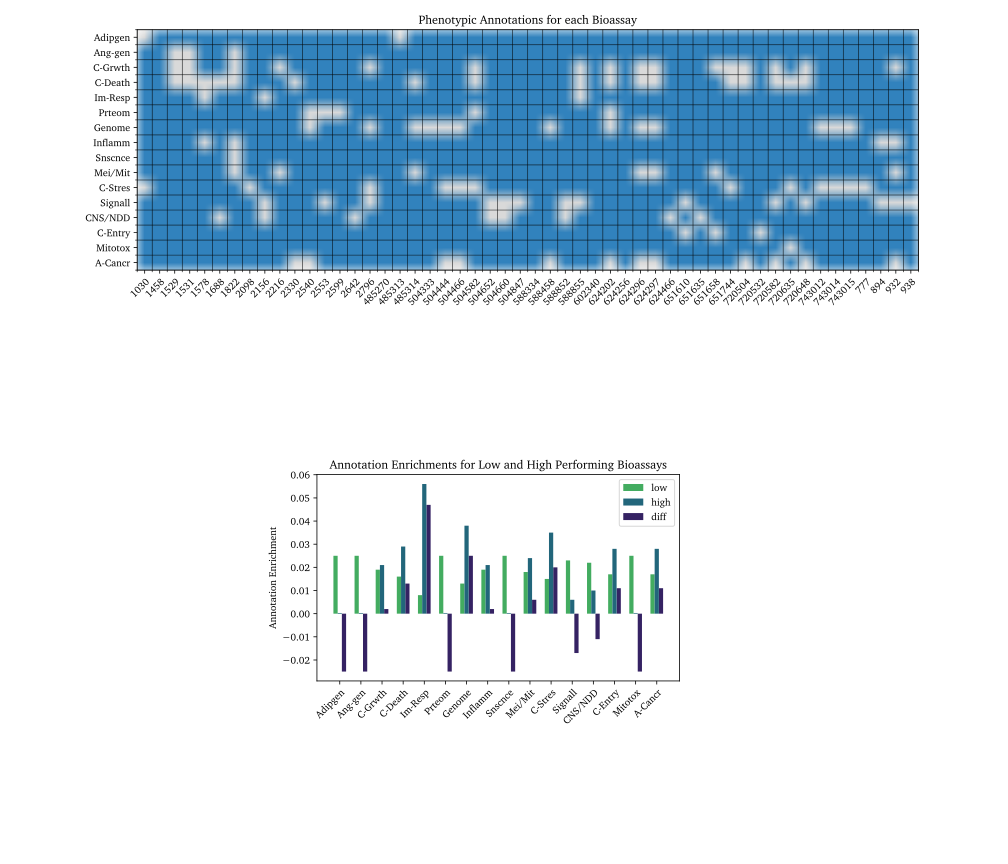
\includegraphics[width=\textwidth]{figures/phenotypic_annotations_corr.pdf}
	\caption[Phenotypic Terms That Can be Associated with Individual \acl{p} Assays]{Phenotypic terms that can be associated with individual \acl{p} assays. These terms were manually filtered from the descriptions of the \acl{p} assays available at \url{https://pubchem.ncbi.nlm.nih.gov/}. White fields correspond to presence and blue entries correspond absence of a term within an assay.}
	\label{fig:phenotypicsparse}
\end{figure}\noindent
Most importantly, the complete annotation matrix was created before the prediction performances were recorded and considered unbiased. This matrix allows testing for enriched annotations within \acl{hpa} and \acl{lpa} respectively.

The state for a phenotypic term within an assay can either be 'present' or 'absent', denoted by a \num{1} or \num{0}. To calculate the partial abundance of a given phenotypic term within a specific assay group $A_p^{xpa}$ the states for all relevant assays $s_p^{(a)}$ are summed up.
\begin{align}\label{eq:phenoabundance}
A_p^{^\text{lpa}} = \sum_{a}^\text{lpa}s_p^{(a)} \quad & A_p^{^\text{hpa}} = \sum_{a}^\text{hpa}s_p^{(a)}
\end{align}
The relative abundances or frequencies $a_p^{xpa}$ with an assay group can be calculated by dividing the partial abundances by the total abundance of the respective phenotypic term.
\begin{align}\label{eq:phenofreq}
a_p^{^\text{lpa}} = \frac{A_p^{^\text{lpa}}}{A_p^{^\text{lpa}}+A_p^{^\text{hpa}}} \quad & a_p^{^\text{hpa}} = \frac{A_p^{^\text{hpa}}}{A_p^{^\text{lpa}} + A_p^{^\text{hpa}}}
\end{align}
The enrichment of phenotypic term within an assay group needs to incorporate the total size of that group $N_{xpa}$. Therefore, the frequencies are divided by the corresponding group size to obtain the term related enrichment $R_p^{^\text{xpa}}$.
\begin{align}\label{eq:phenoenrichment}
R_p^{^\text{lpa}} = \frac{a_p^{^\text{lpa}}}{N_\text{lpa}} \quad & R_p^{^\text{hpa}} = \frac{a_p^{^\text{hpa}}}{N_\text{hpa}}
\end{align}
The resulting measure is the term frequency per assay and describes the enrichment of a phenotypic term within the corresponding assay group.\\
In \fref{tab:phenotypicenrichment} the enrichment for the \acl{hpa} and \acl{lpa} as well as the difference of the two is shown. A negative difference means that this phenotypic term is enriched in the \acl{lpa} and vice versa. It can be seen that phenotypic enrichment is positive for 'C-Grwth', 'C-Death', 'Im-Resp', 'Genome', 'Inflamm', 'Mei/Mit', 'C-Stres', 'C-Entry', and 'A-Cancr'. 'Im-Resp', 'Genome' and 'C-Death' are the three terms showing the highest enrichment.
\begin{figure}[H]
	\centering
	\includegraphics[width=0.9\textwidth]{figures/annotations_enrichment_corr.pdf}
	\caption[Annotations Enrichment in \acl{hpa} and \acl{lpa}]{Annotations Enrichment in \acl{hpa} and \acl{lpa} and the difference of the two. }
	\label{fig:annotenrich}
\end{figure}\noindent

\begin{table}[H]
	\footnotesize
	\centering
	\caption[Enrichment of phenotypic terms in \acl{hpa} and \acl{lpa}]{Enrichment of phenotypic terms in \acl{hpa} and \acl{lpa} and the difference between the two. A high number corresponds to a higher frequency of the corresponding term within the group of assays. The difference clarifies if the relative frequency is higher or lower in the \acl{hpa} and quantifies that enrichment in a comparable manner.}
	\label{tab:phenotypicenrichment}
	\begin{tabularx}{0.95\textwidth}{lllllllll}
		\toprule
		Group & Adipgen & Ang-gen & C-Grwth & C-Death & Im-Resp & Prteom & Genome & Inflamm\\
		\midrule
		low & 0.025 & 0.025 & 0.019 & 0.016 & 0.008 & 0.025 & 0.013 & 0.019\\
		high & 0.0 & 0.0 & 0.021 & 0.029 & 0.056 & 0.0 & 0.038 & 0.021\\
		diff & -0.025 & -0.025 & 0.002 & 0.013 & 0.047 & -0.025 & 0.025 & 0.002\\
		\midrule
		Group & Snscnce & Mei/Mit & C-Stres & Signall & CNS/NDD & C-Entry & Mitotox & A-Cancr\\
		\midrule
		low & 0.025 & 0.018 & 0.015 & 0.023 & 0.022 & 0.017 & 0.025 & 0.017\\
		high & 0.0 & 0.024 & 0.035 & 0.006 & 0.01 & 0.028 & 0.0 & 0.028\\
		diff & -0.025 & 0.006 & 0.02 & -0.017 & -0.011 & 0.011 & -0.025 & 0.011\\
		\bottomrule
	\end{tabularx}
\end{table}\noindent
From this analysis, it can be concluded that assays that probe endpoints related to these specified phenotypes exhibit higher predictive capability with \ac{cp} descriptors. The fact that genome integrity and \ac{dna}-repair scores a high value is also in agreement with the channel enrichment analysis. As shown in \fref{tab:channelstd}, the \ac{dna} channel has the highest ratio among all five.

\section{Gene Ontology Term Analysis}\label{sec:goterms}
% intro
\ac{go} terms are keywords referring to molecular functions or cellular processes associated with proteins. Each protein target is assigned a terminal \ac{go} term that is part of a hierarchical network. Hence every \ac{go} term can be associated with parent \ac{go} terms until the highest level of generalization is reached, leading to a tree of \ac{go} terms that are associated with each known protein.\\
% how they are applied here
%% discuss the six bioassays with no go terms
As an addition to the manually generated phenotypic annotations \ac{go} terms are generated for each bioassay which probes a protein target. Twelve \ac{p} assays do not probe protein targets, six of which are part of the \acl{hpa} group, and they are further discussed below. The terminal \ac{go} terms were obtained from \url{https://www.ebi.ac.uk/interpro} for each target and the entire hierarchy is extracted from \url{http://geneontology.org}. Since \ac{go} terms are hierarchical, a protein target with several unique terminal \ac{go} terms can have duplicate high order \ac{go} terms. For the analysis frequency information, i.e. how often a \ac{go} term appears within a given protein target is discarded. Afterwards, the relative abundance of \ac{go} terms within \acl{hpa} and \acl{lpa} are computed and compared. \ac{go} terms that are only present once throughout all assays are considered too rare to be included in comparative analysis and are therefore discarded. Since the \ac{go} terms directly describe mechanisms within the cell, a deeper understanding of the performances is anticipated. The concept is analogous to the manually developed phenotypic annotations because certain cellular mechanisms are anticipated to be more abundant within a certain group of assays.\\
% describe the figure
All \ac{go} terms found for the \num{52} \ac{p} assays and their relative abundances within high and \acl{lpa} are shown in \fref{fig:gotermabundances}. Roughly a third of the \ac{go} terms are associated with the \acl{hpa} most of which are also more abundant within \acl{hpa}. Furthermore, some of the \ac{go} terms are only present for \acl{hpa}. A majority of the \ac{go} terms found in total are present within protein targets of \acl{lpa}. A considerable amount of these is not present for \acl{hpa}.\\
% shortcomings
One problem that must be addressed concerns the small sample size. The \acl{hpa} only features six protein targets. That means the relative abundances are either \num{1/6}, \num{2/6}, etc. The \acl{lpa} feature this issue to a decreased extent. Therefore, this analysis has to be interpreted with a lack of data fidelity in mind. This approach is considered feasible if the number of biochemical assays is increased.
\begin{figure}[H]
	\centering
	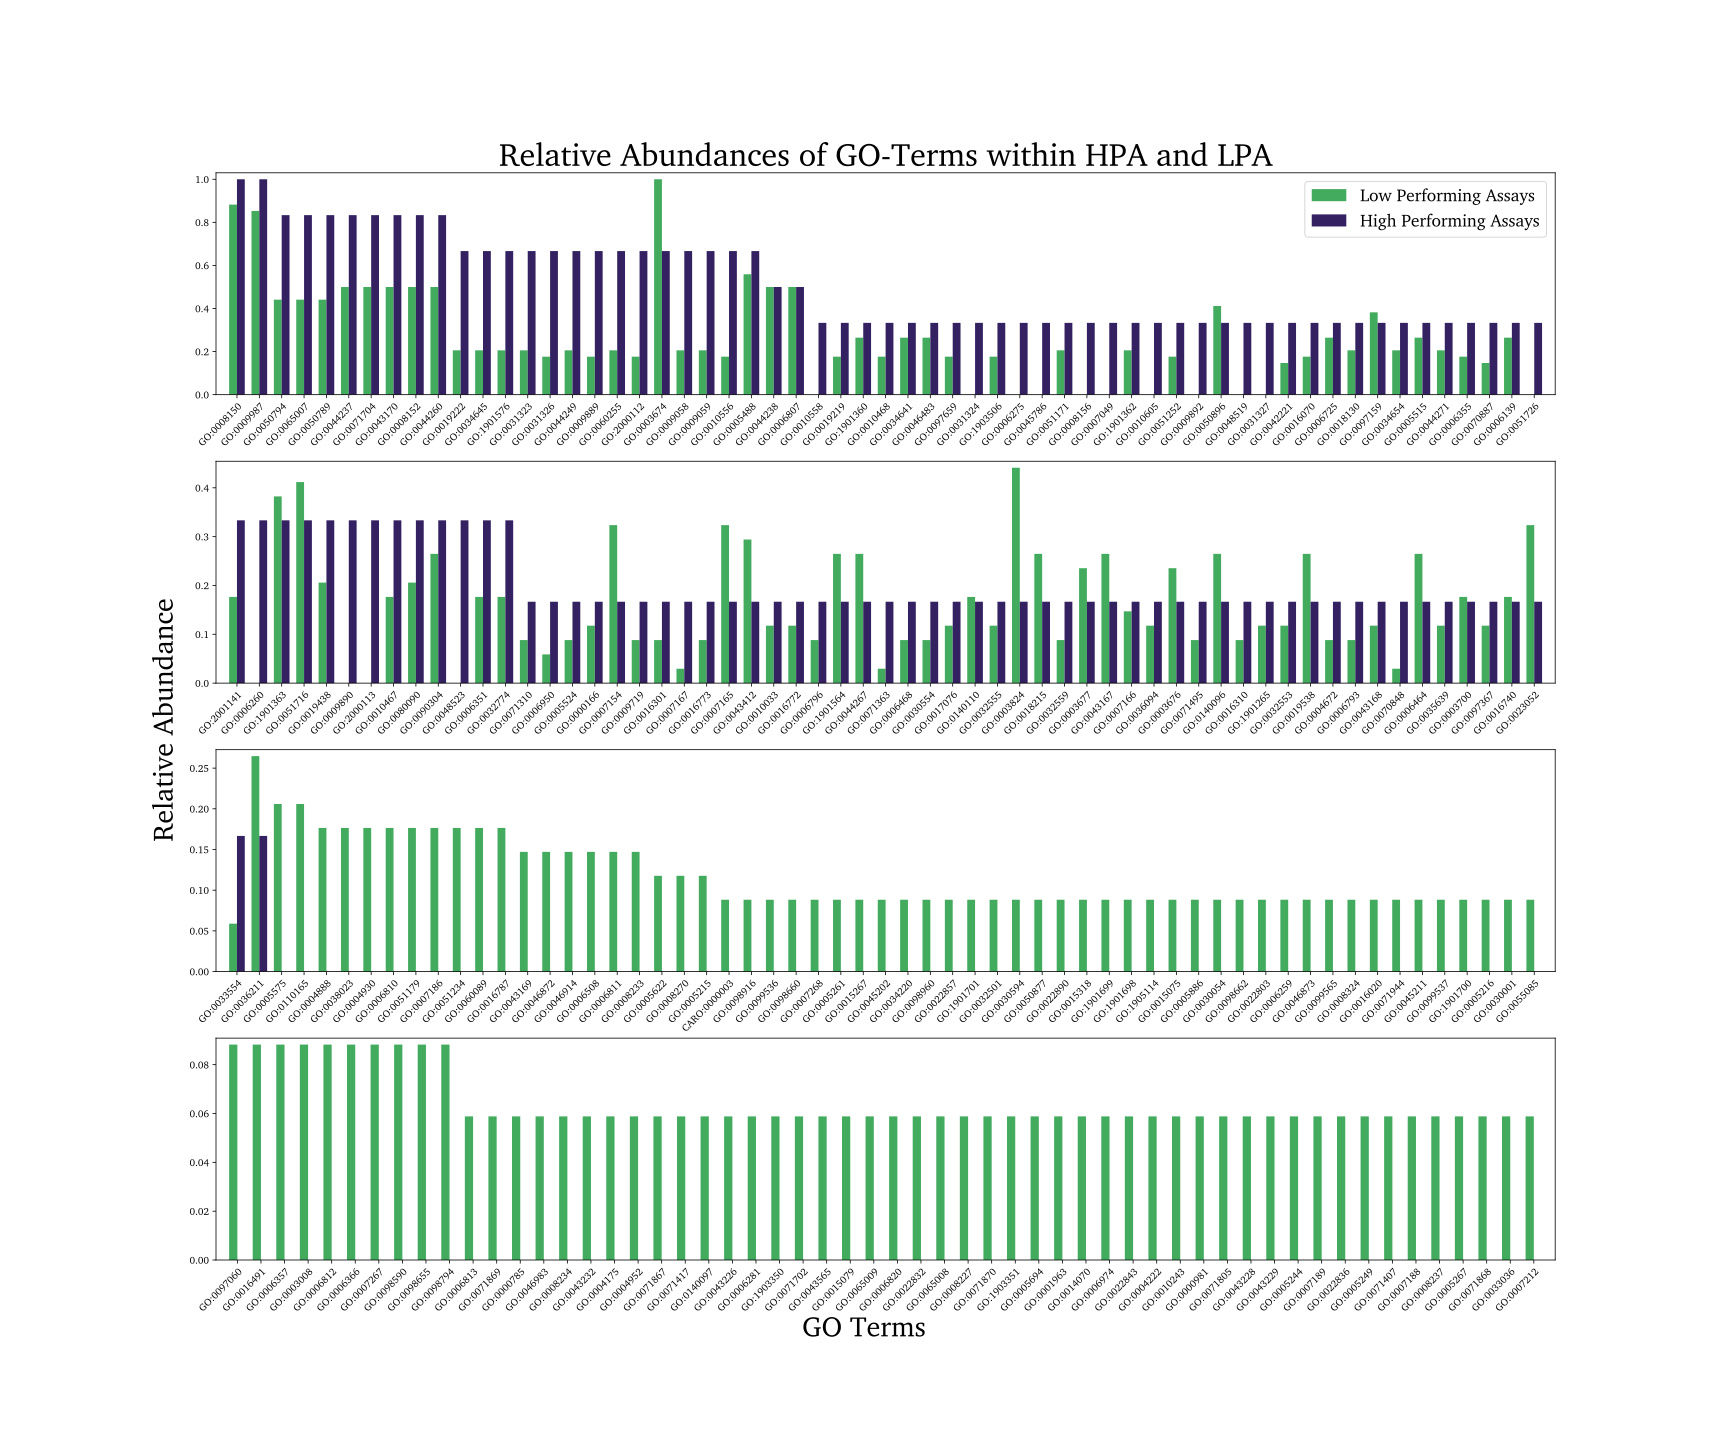
\includegraphics[width=\textwidth]{figures/go_frequencies.pdf}
	\caption[Relative Abundances of \ac{go} Terms in Each Assay Group]{Relative abundances of \ac{go} Terms in each assay group}
	\label{fig:gotermabundances}
\end{figure}
% conclusion
\fref{fig:gotermabundances} serves the sole purpose of visualization since it is only annotated with the \ac{go} term identifier and not with its description. The descriptions for \ac{go} terms enriched in high or \acl{lpa} can be found in \fref{tab:goterms} in the appendix. The \ac{go} terms for \acl{lpa} are very diverse and many instances related to synapses, ion transport and G-protein coupled receptors can be found. For \acl{hpa} the terms are enriched for metabolic and biosynthetic processes of macromolecules as well as the regulation and processing of \ac{dna} and \acs{rna}. This is in agreement with findings from \fref{sec:channelsresults}. In that section, the most important \ac{cp} features are analyzed for enrichment of channel variance. The \ac{dna} channel of \acl{hpa} is enriched by \SI{226}{\percent} compared to \acl{lpa}. Also in \fref{sec:phenotypicannotationsresults} the phenotypic annotation connected to genotoxicity and genetic regulation is highly enriched for \acl{hpa}. \ac{cp} descriptors seem to be particularly sensitive to bioassays primarily related to the regulation and processing of \ac{dna} and \ac{rna}. Nevertheless, the nucleus is the largest organelle in the cell. And the \ac{cp} descriptors are rooted in fluorescence microscopy which is dependend on signal resolution. Since most of the signal that is eventually imaged stems from the nucleus and is therefore related to \ac{dna} and \ac{rna}, this conclusion seems logical.\\
Additionally, the \acl{hpa} that do not probe gene products are inspected in further detail. The assays 651635, 651744, 720532, 743014, 743012 and 743015 are involved. Five out of these six probe complex cellular processes instead of single gene products. 651635 is the only assay that probes a gene product with no \ac{go} terms available by now. In \fref{sec:pubchem} the assay 720532 was explained in further detail as an example because it is the bioassay scoring the highest \ac{auc} via \ac{cp} descriptors. This assay probed the inhibition of virus entry by targeting cellular processes exploited by the virus. 651744 probes cytotoxicity within NIH3T3 cells via luminescence. 743012, 743014 and 743015 are parts of the same experiment where genotoxicity is screened for different mutants of the DT40 cell line.\\
Remarkably, five out of seven bioassays within \acl{hpa} probe for complex cellular processes. On the one hand, this hinders the annotation by \ac{go} terms. On the other hand, this indicates that \ac{cp} contains information that is particularly applicable for more complex cellular processes going beyond molecular functionality. This finding agrees with the richness in information that was also found by Simm \textit{et al.}\cite{Simm2017} when their \ac{cp} based model scored an \ac{auc} greater than \num{0.9} for \num{34} out of \num{600} assay. The authors do not specify what endpoints these assays probe in detail. The execution of an analysis similar to this one could validate the notion that \ac{cp} is most suitable for modelling complex biological mechanisms. 